\chapter{雪盖土壤热力过程}
%\addcontentsline{toc}{chapter}{雪盖土壤热力过程}

%\begin{雪盖土壤热力过程}

在雪盖和土壤中,热力过程主要根据热传导第二定律进行描述。假设雪盖土壤无水平物质能量交换,则其垂直方向上的一维能量平衡方程如下:
\begin{equation}\label{eq:1d_energy_balance}
c \frac{\partial T}{\partial t}=-\frac{\partial F}{\partial z}
\end{equation}
其中$c$表示雪盖或土壤的体积热容量(\unit{J.m^{-3}.K^{-1}}),$T$表示雪盖土壤温度 (K),$t$表示时间(s),$z$表示雪盖高度或土壤深度 (m),
F表示垂直方向的热传导通量,方向向上为正(\unit{W.m^{-2}}),表达式为$F=-\lambda\frac{\partial T}{\partial z}$,$\lambda$表示热力传导率(\unit{W.m^{-1}.K^{-1}})。
将方程(\ref{eq:1d_energy_balance})进行离散,并结合上边界由大气输送到雪盖土壤表面的热通量$h_s$以及下边界土壤底层的零热通量,
即可求出雪盖土壤的温度廓线,之后再根据相态变化条件对温度进行进一步调整。


\section{温度求解的数值格式}\label{温度求解的数值格式}

\begin{mymdframed}{代码}
本节对应的代码文件为\texttt{MOD\_GroundTemperature.F90}。
\end{mymdframed}

在离散上述能量平衡方程时,垂直方向上的离散方式可采用第~\ref{土壤和积雪的垂直分层} 节给出的土壤和积雪的垂直分层方案进行。
需要额外注意的是,在计算雪盖土壤温度之前,若有降雪发生($p_i>0$)且无雪盖分层($snl=0$),则此时需通过下式判断第一层雪能否形成:
\begin{equation}
\begin{aligned}
z_{sno} &= z_{sno}+\frac{p_{i} \Delta t}{\rho_{\text {sno,new }}} \\[1ex] 
W_{sno} &= W_{sno}+p_{i} \Delta t
\end{aligned}
\end{equation}
其中$\rho_{sno,new}$表示新降的干雪密度(\unit{kg.m^{-3}}),计算方案为~\citep{anderson1976point}:
\begin{equation}
\rho_{sno, new}=\begin{cases}
169 & \text { 当 }\ T_{atm}>T_{f}+2.0 \\ 
50+1.7\left(T_{atm}-T_{f}+15\right)^{1.5}  & \text { 当 }\ T_{f}-15.0<T_{atm} \leqslant T_{f}+2.0 \\ 
50 & \text { 当 }\ T_{atm} \leqslant T_{f}-15.0
\end{cases}
\end{equation}
若此时$z_{sno} \geqslant 0.01$,则按第~\ref{土壤和积雪的垂直分层} 节方案对积雪进行分层,且每一层雪的温度取为$T_p$,液态水含量取为0,固态水含量按雪层厚度权重分配$W_{sno}$。若之前已有雪层且此时有降雪发生,则第一层雪的相关物理量作如下更新:
\begin{equation}
w_{ice, snl+1}=w_{ice, snl+1}+p_{i} \Delta t
\end{equation}
\begin{equation}
\Delta z_{snl+1}=\Delta z_{snl+1}+\frac{p_{i} \Delta t}{\rho_{sno, new}}
\end{equation}
\begin{equation}
z_{snl+1}=z_{h, snl+1}-0.5 \Delta z_{snl+1}
\end{equation}
\begin{equation}
z_{h, snl}=z_{h, snl+1}-\Delta z_{snl+1}
\end{equation}
雪盖土壤垂直分层及其热传导过程示意图见图~\ref{fig:雪盖土壤垂直分层及其热传导过程示意图}。其中土壤热力学状态变量
(如雪盖土壤温度$T_i$,热力传导率$\lambda_i$,体积比热容$c_i$等)定义在每一层的中间深度,从第$i+1$层到第$i$层的热传导通量$F_i$定义在两层的交界处,它可离散为:
\begin{equation}
F_{i}=\lambda\left[z_{h, i}\right] \frac{T_{i}-T_{i+1}}{z_{i}-z_{i+1}}
\end{equation}
其中$\lambda\left[z_{h,i}\right]$表示第$i+1$层与第 $i$ 层交界处的热力传导率。求解$\lambda\left[z_{h,i}\right]$时,
假设从第$i+1$层到第$i$层的热传导通量等于从第$i+1$层到第$i+1$层与第$i$层交界层的热传导通量,又等于从交接层到第$i$层的热传导通量,即
\begin{equation}
\lambda\left[z_{h, i}\right] \frac{T_{i}-T_{i+1}}{z_{i}-z_{i+1}}=\lambda_{i+1} \frac{T_{m}-T_{i+1}}{z_{h, i}-z_{i+1}}=\lambda_{i} \frac{T_{i}-T_{m}}{z_{i}-z_{h, i}}
\end{equation}
即可通过后两项解出第$i+1$层与第$i$层交界处的温度$T_m$;再将$T_m$代回,通过前两项即可解出$\lambda\left[z_{h,i}\right]$为:
\begin{equation}
\lambda\left[z_{h, i}\right]=\begin{cases}
\frac{\lambda_{i} \lambda_{i+1}\left(z_{i}-z_{i+1}\right)}{\lambda_{i}\left(z_{h, i}-z_{i+1}\right)+\lambda_{i+1}\left(z_{i}-z_{h, i}\right)} & i=snl+1, \ldots, 9 \\ 
0 & i=10
\end{cases}
\end{equation}
特殊地,对于土壤与雪盖的交界面,为防止最下层雪盖厚度过大导致$\lambda\left[z_{h,i}\right]$计算不准,
当$i=0$且$\left(z_{i+1}-z_{h,i}\right)<\left(z_{h,i}-z_i\right)$时,$\lambda\left[z_{h,i}\right]$重新计算为:
\begin{equation}
\lambda\left[z_{h,i}\right]=\frac{2 \lambda_{i} \lambda_{i+1}}{\lambda_{i}+\lambda_{i+1}} \geqslant 0.5 \lambda_{i+1}
\end{equation}
{
\begin{figure}[htbp]
\centering
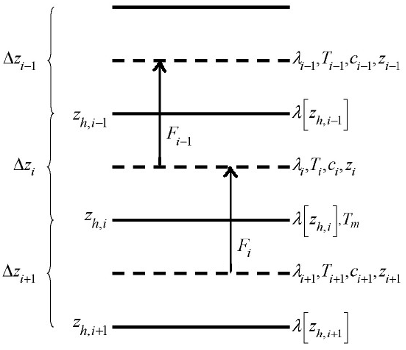
\includegraphics{Figures/雪盖土壤热力过程/雪盖土壤垂直分层及其热传导过程示意图.png}
\caption{雪盖土壤垂直分层及其热传导过程示意图}
\label{fig:雪盖土壤垂直分层及其热传导过程示意图}
\end{figure}
}


基于以上离散方案,第$i$层雪盖土壤的能量平衡方程可表达为:
\begin{equation}
\frac{c_{i} \Delta z_{i}}{\Delta t}\left(T_{i}^{n+1}-T_{i}^{n}\right)=F_{i}-F_{i-1}
\end{equation}
%
其中$\Delta t$表示积分时间步长,$n$表示积分步数。此方程采用Crank--Nicholson半隐式格式求解,既包含前一时刻已有的温度与热通量信息,又包含后一时刻的预报信息。于是此方程可写为如下形式:
\begin{equation}
\frac{c_{i} \Delta z_{i}}{\Delta t}\left(T_{i}^{n+1}-T_{i}^{n}\right)=\alpha\left(F_{i}^{n}-F_{i-1}^{n}\right)+(1-\alpha)\left(F_{i}^{n+1}-F_{i-1}^{n+1}\right)
\end{equation}
其中权重因子$\alpha=0.5$。此方程展开,即有
\begin{equation}
\begin{aligned} 
\frac{c_{i} \Delta z_{i}}{\Delta t}\left(T_{i}^{n+1}-T_{i}^{n}\right)=& 0.5\left\{\lambda\left[z_{h, i}\right] \frac{T_{i}^{n}-T_{i+1}^{n}}{z_{i}-z_{i+1}}-\lambda\left[z_{h, i-1}\right] \frac{T_{i-1}^{n}-T_{i}^{n}}{z_{i-1}-z_{i}}\right.\\[1ex] &\left.+\lambda\left[z_{h, i}\right] \frac{T_{i}^{n+1}-T_{i+1}^{n+1}}{z_{i}-z_{i+1}}-\lambda\left[z_{h, i-1}\right] \frac{T_{i-1}^{n+1}-T_{i}^{n+1}}{z_{i-1}-z_{i}}\right\} 
\end{aligned}
\end{equation}
将所有层雪盖土壤能量平衡方程联立,可形成关于预报变量$T_{i-1}^{n+1}$,$T_i^{n+1}$和$T_{i+1}^{n+1}$的三对角方程组形式:$r_i=a_iT_{i-1}^{n+1}+b_iT_i^{n+1}+c_iT_{i+1}^{n+1}$,
其中$a_i$, $b_i$, $c_i$分别为三对角矩阵中上三角、对角线和下三角位置中的元素。用追赶法解此方程组即可快速求得每一层雪盖土壤的温度$T_i^{n+1}$。


对于雪盖土壤的中间层($snl+1<i<10$),三对角矩阵中的系数表达如下:
\begin{equation}
\begin{aligned}
a_{i} &= -(1-\alpha) \frac{\Delta t}{c_{i} \Delta z_{i}} \frac{\lambda\left[z_{h, i-1}\right]}{z_{i}-z_{i-1}} \\[1ex] 
b_{i} &= 1+(1-\alpha) \frac{\Delta t}{c_{i} \Delta z_{i}}\left[\frac{\lambda\left[z_{h, i-1}\right]}{z_{i}-z_{i-1}}+\frac{\lambda\left[z_{h, i}\right]}{z_{i+1}-z_{i}}\right] \\[1ex] 
c_{i} &= -(1-\alpha) \frac{\Delta t}{c_{i} \Delta z_{i}} \frac{\lambda\left[z_{h, i}\right]}{z_{i+1}-z_{i}} \\[1ex]
r_{i} &= T_{i}^{n}+\alpha \frac{\Delta t}{c_{i} \Delta z_{i}} \lambda\left[z_{h, i}\right] \frac{T_{i}^{n}-T_{i+1}^{n}}{z_{i}-z_{i+1}}-\lambda\left[z_{h, i-1}\right] \frac{T_{i-1}^{n}-T_{i}^{n}}{z_{i-1}-z_{i}}
\end{aligned}
\end{equation}

对于雪盖土壤的顶层和底层,需要考虑对应的边界条件:

(1) 对于雪盖土壤顶层($i=snl+1$),来自大气的热通量$h_s$将会进入到地表中,即
\begin{equation}
h_{s}^{n+1}=-\alpha F_{i-1}^{n}-(1-\alpha) F_{i-1}^{n+1}
\end{equation}
对$h_s^{n+1}$采用一阶泰勒展开近似,则顶层能量平衡方程变为:
\begin{equation}
\begin{split}
&\mathrel{\phantom{\approx}}\frac{c_{i} \Delta z_{i}}{\Delta t}\left(T_{i}^{n+1}-T_{i}^{n}\right)=h_{s}^{n+1}+\alpha F_{i}^{n}+(1-\alpha) F_{i}^{n+1} \\[1ex] 
&\approx h_{s}^{n}+\frac{\partial h_{s}}{\partial T_{i}}\left(T_{i}^{n+1}-T_{i}^{n}\right)+\alpha \lambda\left[z_{h, i}\right] \frac{T_{i}^{n}-T_{i+1}^{n}}{z_{i}-z_{i+1}}+(1-\alpha) \lambda\left[z_{h, i}\right] \frac{T_{i}^{n+1}-T_{i+1}^{n+1}}{z_{i}-z_{i+1}}
\end{split}
\end{equation}
于是,基于此方程可得雪盖土壤顶层的三对角矩阵系数为:
\begin{equation}
\begin{aligned}
a_{i} &= 0 \\[1ex] 
b_{i} &= 1+\frac{\Delta t}{c_{i} \Delta z_{i}}\left[(1-\alpha) \frac{\lambda\left[z_{h, i}\right]}{z_{i+1}-z_{i}}-\frac{\partial h_{s}}{\partial T_{i}}\right] \\[1ex]
c_{i} &= -(1-\alpha) \frac{\Delta t}{c_{i} \Delta z_{i}} \frac{\lambda\left[z_{h, i}\right]}{z_{i+1}-z_{i}} \\[1ex]
r_{i} &= T_{i}^{n}+\frac{\Delta t}{c_{i} \Delta z_{i}}\left[h_{s}^{n}-\frac{\partial h_{s}}{\partial T_{i}} T_{i}^{n}+\alpha \lambda\left[z_{h, i}\right] \frac{T_{i}^{n}-T_{i+1}^{n}}{z_{i}-z_{i+1}}\right]
\end{aligned}
\end{equation}
这里进入到地表的热通量$h_s$ (\unit{W.m^{-2}})具体表达为:
\begin{equation}
\begin{aligned}
h_{s} &= S_{g}+L_{g}\left(T_{g}\right)-H_{g}\left(T_{g}\right)-\lambda E_{g}\left(T_{g}\right)+H_{p r c g}\left(T_{g}\right) \\[1.5ex]
\frac{\partial h_{s}}{\partial T_{g}} &= \frac{\partial L_{g}}{\partial T_{g}}-\frac{\partial H_{g}}{\partial T_{g}}-\frac{\partial \lambda E_{g}}{\partial T_{g}}+\frac{\partial H_{p r c g}}{\partial T_{g}}
\end{aligned}
\end{equation}
其中$S_g$和$L_g$分别表示地表吸收的净太阳辐(公式~\eqref{eq:sg})和净长波辐射(公式~\eqref{eq:lg1}, \eqref{eq:lg2}) [\unit{W.m^{-2}}]。$h_s$中感热$H_{g}$和潜热$\lambda E_g$的计算见第~\ref{ch:地表湍流通量} 章,雨水感热$H_{prcg}$的计算见章节~\ref{植被地表的雨水感热}。

另外,对于潜热通量系数$\lambda$,当雪盖土壤顶层不存在液态水时,$\lambda$取为升华潜热系数$\lambda_s$,即:
\begin{equation}
\lambda=\left\{\begin{array}{lr}\lambda_{s} & \text { 当 }\ w_{liq, s n l+1}=0 \text { 并且 }\ w_{ice, s n l+1}>0 \\ \lambda_{v} & \text { 其他情况 }\end{array}\right.
\end{equation}
其中$w_{liq,snl+1}$和$w_{ice,snl+1}$分别表示雪盖土壤顶层的液态水和固态水含量 (\unit{kg.m^{-2}},其计算见第~\ref{积雪和土壤中水分的垂直运动}~章)。

在模式中,地表温度$T_g$与$T_{snl+1}$取为同一值,但$T_{snl+1}$表示第一层雪盖或土壤的平均温度,与实际的$T_g$相比具有减弱的日变化幅度。
为改进这一缺陷,在求解第一层能量平衡方程时,其厚度$\Delta z_i$作以下调整,以求得更接近实际的$T_g$:
\begin{equation}
\Delta z_{i}=0.5\left[z_{i}-z_{h, i-1}+c_{a}\left(z_{i+1}-z_{h, i-1}\right)\right]
\end{equation}
其中调整参数$c_a=0.34$。

(2) 对于土壤底层($i=10$),假设热传导通量为0,则能量平衡方程变为:
\begin{equation}
\frac{c_{i} \Delta z_{i}}{\Delta t}\left(T_{i}^{n+1}-T_{i}^{n}\right)=-\alpha \lambda\left[z_{h, i-1}\right] \frac{T_{i-1}^{n}-T_{i}^{n}}{z_{i-1}-z_{i}}-(1-\alpha) \lambda\left[z_{h, i-1}\right] \frac{T_{i-1}^{n+1}-T_{i}^{n+1}}{z_{i-1}-z_{i}}
\end{equation}
于是,基于此方程可得土壤底层的三对角矩阵系数为:
\begin{equation}
\begin{aligned}
a_{i} &= -(1-\alpha) \frac{\Delta t}{c_{i} \Delta z_{i}} \frac{\lambda\left[z_{h, i-1}\right]}{z_{i}-z_{i-1}} \\
b_{i} &= 1+(1-\alpha) \frac{\Delta t}{c_{i} \Delta z_{i}} \frac{\lambda\left[z_{h, i-1}\right]}{z_{i}-z_{i-1}} \\
c_{i} &= 0 \\
r_{i} &= T_{i}^{n}-\alpha \frac{\Delta t \lambda\left[z_{h, i-1}\right]}{c_{i} \Delta z_{i}} \frac{T_{i-1}^{n}-T_{i}^{n}}{z_{i-1}-z_{i}}
\end{aligned}
\end{equation}

各层雪盖土壤的热力传导率与体积热容量的计算方案将在~\ref{sec_thermalpar} 节给出。


\section{温度的相态变化调整}

\begin{mymdframed}{代码}
本节对应的代码文件为\texttt{MOD\_PhaseChange.F90}。
\end{mymdframed}

通过解能量平衡方程组计算出下一时刻的雪盖土壤温度后,需要考虑相态变化过程对温度进行调整。在模式中,相态变化发生的条件为:\\
若$T_i^{n+1}>T_f$并且$w_{ice,i}>0$ \ \   \ \  \ \   固态水融化\\
若$T_i^{n+1}<T_f$并且$w_{liq,i}>0$  \ \   \ \  \ \         液态水冻结

一个特殊情况是,当土壤表面积雪存在 ($W_{sno}>0$) 但并无雪层($snl=0$,$z_{sno}<0.01$) 时,\\
若$T_1^{n+1}>T_f$      \ \   \ \  \ \                 积雪融化\\
%
以上三种情况下,$T_i^{n+1}$被调整为$T_f$。


相态变化的程度是由$T_i^{n+1}$调整为$T_f$后产生的能量冗余或亏损决定的。温度调整后,能量的冗余或亏损$H_i$ (\unit{W.m^{-2}})计算如下:
\begin{equation}
H_{i}=\begin{cases}
h_{s}^{n}+\frac{\partial h_{s}}{\partial T_{i}}\left(T_{f}-T_{i}^{n}\right)+\alpha F_{i}^{n}+(1-\alpha) F_{i}^{n+1}-\frac{c_{i} \Delta z_{i}}{\Delta t}\left(T_{f}-T_{i}^{n}\right) & i=snl+1 \\
\alpha\left(F_{i}^{n}-F_{i-1}^{n}\right)+(1-\alpha)\left(F_{i}^{n+1}-F_{i-1}^{n+1}\right)-\frac{c_{i} \Delta z_{i}}{\Delta t}\left(T_{f}-T_{i}^{n}\right) & snl+1<i<10 \\
-\alpha F_{i-1}^{n}-(1-\alpha) F_{i-1}^{n+1}-\frac{c_{i} \Delta z_{i}}{\Delta t}\left(T_{f}-T_{i}^{n}\right) & i=10
\end{cases}
\end{equation}
对应地,相态变化的质量调整量为$H_{m}=\frac{H_{i} \Delta t}{L_{f}}$,其中$L_f$表示固态水液化潜热(\unit{J.kg^{-1}})。当固态水融化条件被满足且$H_m>0$时,固态水含量被调整为:
\begin{equation}
w_{ice, i}^{n+1}=w_{ice, i}^{n}-H_{m} \geqslant 0
\end{equation}
当液态水冻结条件被满足且$H_m<0$时,固态水含量被调整为:
\begin{equation}
w_{ice, i}^{n+1}=\min{\left(w_{ice, i}^{n}-H_{m}, w_{liq, i}^{n}+w_{ice, i}^{n}\right)}
\end{equation}
以上情况液态水含量均被调整为:
\begin{equation}
w_{liq, i}^{n+1}=w_{liq, i}^{n}+w_{ice, i}^{n}-w_{ice, i}^{n+1} \geqslant 0
\end{equation}
若水分调节过程不足以消耗全部的能量冗余或填补全部的能量亏损,
则在相态变化过程之后再次进行能量结余计算:$ H_{i *}=H_{i}+\frac{L_{f}\left(w_{ice, i}^{n+1}-w_{ice, i}^{n}\right)}{\Delta t}$。
若$\left|H_{i\ast}\right|>0$,则此部分能量可用来再次暖化或冷却雪盖土壤层,温度调整如下:
\begin{equation}
T_{i}^{n+1}=\left\{\begin{array}{lr}T_{f}+\frac{\Delta t}{c_{i} \Delta z_{i}} H_{i *} /\left(1-\frac{\Delta t}{c_{i} \Delta z_{i}} \frac{\partial T_{s}}{\partial T_{i}}\right) & i=s n l+1 \\ T_{f}+\frac{\Delta t}{c_{i} \Delta z_{i}} H_{i *} & i \neq s n l+1 \\ T_{f} & w_{liq, i}^{n+1} \cdot w_{ice, i}^{n+1}>0\end{array}\right.
\end{equation}
对于特殊的土壤表面积雪融化的情形,当$H_m>0$时,雪水当量减少为
\begin{equation}
W_{sno}^{n+1}=W_{s no}^{n}-H_{m} \geqslant 0
\end{equation}
同样,雪的厚度减少为
\begin{equation}
z_{sno}^{n+1}=\frac{W_{sno}^{n+1}}{W_{sno}^{n}} z_{sno}^{n}
\end{equation}
若积雪融化不足以消耗全部的能量冗余,则剩余能量$H_{1\ast}$为
\begin{equation}
H_{1 *}=H_{1}+\frac{L_{f}\left(W_{sno}^{n+1}-W_{sno}^{n}\right)}{\Delta t}
\end{equation}
此时$H_{1\ast}$将作为新的$H_1$对第一层土壤进行上述相态变化计算。


综上,若发生土壤表面积雪融化的情形,则用于相态变化的能量累计$E$为:
\begin{equation}
E=\frac{L_{f}\left(W_{sno}^{n}-W_{sno}^{n+1}\right)}{\Delta t}+\sum_{i=1}^{10} \frac{L_{f}\left(w_{ice, i}^{n}-w_{ice, i}^{n+1}\right)}{\Delta t}
\end{equation}
否则,
\begin{equation}
E=\sum_{i=1}^{s n l+1} \frac{L_{f}\left(w_{ice, i}^{n}-w_{ice, i}^{n+1}\right)}{\Delta t}
\end{equation}
以上过程即是雪盖土壤温度计算的全部过程。得到$T_i^{n+1}$后,地表发出的上行长波辐射$L_g\uparrow$,感热通量$H_g$与潜热通量$\lambda E_g$需再做一次更新以作为输出的状态变量,
其中用于蒸发的水汽不能超过雪盖土壤顶层的总含水量$\left(w_{liq,snl+1}^{n+1}+w_{ice,snl+1}^{n+1}\right)/\Delta t$,
否则地表蒸发水汽取为$\left(w_{liq,snl+1}^{n+1}+w_{ice,snl+1}^{n+1}\right)/\Delta t$,产生的能量误差将加到感热通量上。


\section{雪盖土壤热力参数的计算方案}\label{sec_thermalpar}
\begin{mymdframed}{代码}
本节对应的代码文件为\texttt{MOD\_SoilThermalParameters.F90}。
\end{mymdframed}

雪盖土壤的热力参数是完成雪盖土壤热力过程数值模拟、求解前文所述垂直方向能量平衡方程的必要输入参数,主要包含两类:雪盖土壤的体积热容量和导热率。下面就这两类参数给出在CoLM中的计算方案。

\subsection{雪盖土壤的体积热容量}

体积热容量的计算较为简单。根据 \citet{de1963thermal},土壤体积热容量由固体土壤、液态水和固态水的热容量基于各自的体积百分比加权平均得到,表达为:
\begin{equation}
c_{i}=c_{s, i}\left(1-\theta_{s, i}\right)+\frac{w_{ice, i}}{\Delta z_{i}} C_{pi}+\frac{w_{liq, i}}{\Delta z_{i}} C_{p l}
\end{equation}
其中$c_{s,i}$表示第$i$层的固体土壤体积热容量,由地表参数数据集提供。若地表有积雪但无雪层,则积雪的热容量也需考虑:
\begin{equation}
c_{i}=c_{s,i}\left(1-\theta_{s, i}\right)+\frac{w_{ice, i}}{\Delta z_{i}} C_{pi}+\frac{w_{liq,i}}{\Delta z_{i}} C_{pl}+\frac{W_{sno}}{\Delta z_{i}} C_{pi}
\end{equation}
其中,固体土壤假设由矿物质土壤、有机质土壤和砾石组成,每种成分的体积热容量基于各自的体积百分比加权平均即得到固体土壤的体积热容量。有机质土壤和砾石的体积热容量分别取值为$2.51\times 10^6$ \unit{J.m^{-3}.K^{-1}}和$2.35\times 10^6$ \unit{J.m^{-3}.K^{-1}},矿物质土壤的体积热容量(\unit{J.m^{-3}.K^{-1}})由如下方案给出:$$c_{minerals}=\frac{2.128\times\%sand+2.385\times\%clay}{\%sand+\%clay}\times10^6$$ 
其中$\%sand$和$\%clay$表示沙土和黏土的质量百分比。

雪盖体积热容量由液态水和固态水的热容量基于各自的体积百分比加权平均得到,表达为:
\begin{equation}
c_{i}=\frac{w_{ice, i}}{\Delta z_{i}} C_{pi}+\frac{w_{liq, i}}{\Delta z_{i}} C_{pl}
\end{equation}
其中,液态水和固态水的热容量可参见表~\ref{tab:物理常数}。

\subsection{雪盖土壤的导热率}

在CoLM中,土壤导热率(\unit{W.m^{-1}.K^{-1}})引入了8种计算方案供用户选择,分别为:\citet{Johansen1975}方案及其5个衍生方案(\citet{farouki1981thermal}, \citet{cote2005}, \citet{balland2005},\citet{lu2007improved}和~\citet{Yan2019thermal}),一个经验方案(\citet{tarnawski2012series})和一个理论方案(\citet{de1963thermal})。以上方案均在各自原始方案基础上,假设固体土壤由矿物质土壤、有机质土壤和砾石组成的前提下进行了改进。根据\citep{dai2019evaluation}在一定观测样本下的评估结果,\citet{balland2005}方案的模拟性能相对较优,故设为默认方案。下面将给出以上8种方案的具体计算方法。

\subsubsection{\citet{Johansen1975}方案}
\citet{Johansen1975}将土壤导热率$k$视为干土壤导热率$k_{dry}$和饱和土壤导热率$k_{sat}$的线性组合,其中饱和土壤导热率的权重系数为$K_e$(称为Kersten数)。于是,土壤导热率可表达为:
\begin{equation}\label{eq:STC}
k=(k_{sat}-k_{dry})K_e+k_{dry}
\end{equation}
其中,$K_e$可视为土壤饱和度$S_r$(定义为实际土壤含水量与饱和土壤含水量的比值)、土壤水相态和土壤粒径的函数,计算为:
\begin{equation}
K_e=\begin{cases}
0.7\log_{10}S_r+1 & \text {对于粗质颗粒的未冻结土壤且}\ Sr>0.05\ \text {时} \\ 
\log_{10}S_r+1 & \text {对于细质颗粒的未冻结土壤且}\ Sr>0.1\ \text {时} \\ 
S_r & \text {对于冻结土壤时}
\end{cases}
\end{equation}

在方程~\eqref{eq:STC} 中,干土壤导热率$k_{dry}$由固体土壤各成分导热率基于其在固体土壤中的体积分数进行算术加权平均得到,计算表达式为:
\begin{equation}\label{eq:STC_dry}
k_{dry}=f_{minerals}k_{minerals\_dry}+f_{om}k_{om\_dry}+f_{gravel}k_{gravel\_dry}
\end{equation}
其中,$f_{minerals}$,$f_{om}$和$f_{gravel}$分别表示矿物质土壤、有机质土壤和砾石在固体土壤中的体积分数;$k_{om\_dry}$和$k_{gravel\_dry}$分别表示有机质土壤和砾石在干燥状态下的整体导热率,取值为$k_{om\_dry}=0.05$,$k_{gravel\_dry}=0.039\theta_s^{-2.2}$($\theta_s$表示土壤孔隙度);$k_{minerals\_dry}$表示矿物质土壤在干燥状态下的导热率,计算为:$$k_{minerals\_dry}=\frac{0.135\rho_d+0.0647}{2.7-0.947\rho_d}$$
$\rho_d$表示矿物质土壤的干容重(\unit{g.cm^{-3}})。

饱和土壤导热率$k_{sat}$由固体土壤各成分导热率和水(冰)导热率基于其体积分数进行几何加权平均得到,计算表达式为:
\begin{equation}\label{eq:STC_wet}
k_{sat}=k_{minerals\_wet}^{v_m}k_{om\_wet}^{v_{om}}k_{gravel\_wet}^{v_g}k_w^{\theta_s}
\end{equation}
其中,$v_m$,$v_{om}$和$v_g$分别表示矿物质土壤、有机质土壤和砾石在整体土壤柱内的体积分数;$k_{minerals\_wet}$,$k_{om\_wet}$和$k_{gravel\_wet}$分别表示矿物质土壤、有机质土壤和砾石在饱和土壤状态下的整体导热率,$k_w$表示水(冰)的导热率(参见表~\ref{tab:物理常数})。$k_{om\_wet}$和$k_{gravel\_wet}$分别取值为0.25和2.875;$k_{minerals\_wet}$由矿物质土壤中石英部分导热率$k_q$与非石英部分导热率$k_o$基于其在矿物质土壤中的体积分数进行几何加权平均得到:$$k_{minerals\_wet}=k_q^{v_q}k_o^{1-v_q}$$
其中,$k_q$取值为7.7,$k_o$依据石英的体积分数$v_q$决定:
\begin{equation}
k_o=\begin{cases}
2.0 & \text {当}\ v_q>0.2\ \text {时} \\ 
3.0 & \text {当}\ v_q\leqslant 0.2\ \text {时}
\end{cases}
\end{equation}
$v_q$可由~\citet{PL_98}基于12种土壤类型(依据美国农业部USDA的土壤质地分类标准)给出的经验值查表获得。

\subsubsection{\citet{farouki1981thermal}方案}
\citet{farouki1981thermal}方案作为~\citet{Johansen1975}方案的衍生方案,土壤导热率$k$与干土壤导热率$k_{dry}$的计算方式完全一致(\eqref{eq:STC} 和~\eqref{eq:STC_dry})。饱和土壤导热率$k_{sat}$由固体土壤导热率和水(冰)导热率基于其体积分数进行几何加权平均得到,而固体土壤导热率取值为各成分导热率基于其在固体土壤中的体积分数的算术加权平均值。$k_{sat}$计算表达式为:
\begin{equation}\label{eq:STC_wet_Farouki}
k_{sat}=(f_{minerals}k_{minerals\_wet}+f_{om}k_{om\_wet}+f_{gravel}k_{gravel\_wet})^{1-\theta_s}k_w^{\theta_s}
\end{equation}
其中,$k_{minerals\_wet}$也与~\citet{Johansen1975}方案的计算方式不同,表达为:$$k_{minerals\_wet}=\frac{8.80\times\%sand+2.92\times\%clay}{\%sand+\%clay}$$ 
其中$\%sand$和$\%clay$表示沙土和黏土的质量百分比。

Kersten数$K_e$的计算方式相较~\citet{Johansen1975}方案更为简化,表达为:
\begin{equation}
K_e=\begin{cases}
\log_{10}S_r+1 & \text {对于未冻结土壤时} \\ 
S_r & \text {对于冻结土壤时}
\end{cases}
\end{equation}

\subsubsection{\citet{cote2005}方案}
在~\citet{cote2005}方案中,土壤导热率$k$与饱和土壤导热率$k_{sat}$的计算方式与~\citet{Johansen1975}方案完全一致(\eqref{eq:STC} 和~\eqref{eq:STC_wet})。而干土壤导热率$k_{dry}$和Kersten数$K_e$的计算方案则通过大量实测数据拟合得到经验关系式。$k_{dry}$表达为:
\begin{equation}\label{eq:STC_dry_CK}
k_{dry}=\sum_if_i\chi_i(10^{-\eta_i\theta_s}),\quad i=\text{矿物质土壤、有机质土壤或砾石}
\end{equation}
$K_e$表达为:
\begin{equation}
K_e=\frac{\kappa S_r}{1+(\kappa -1)S_r}
\end{equation}
其中$\chi_i$、$\eta_i$和$\kappa$为经验参数,按照表~\ref{tab:Cote2005方案中k计算参数取值} 和~\ref{tab:Cote2005方案中k计算参数kappa取值} 取值:
\begin{table}[htbp]
    \centering
    \caption{\citet{cote2005}方案中$k_{dry}$计算公式中的参数取值}
    \label{tab:Cote2005方案中k计算参数取值}
    \begin{tabular}{@{}lcc@{}}
    \toprule
    土壤成分               & $\chi$     & $\eta$  \\
    \midrule
    砾石                  & 1.70      & 1.80  \\
    有机质土壤                  & 0.30    & 0.87   \\
    矿物质土壤         & 0.75   & 1.20    \\
    \bottomrule
    \end{tabular}
\end{table}
%
\begin{table}[htbp]
    \centering
    \caption{\citet{cote2005}方案中$K_e$计算公式中$\kappa$的参数取值}
    \label{tab:Cote2005方案中k计算参数kappa取值}
    \begin{tabular}{@{}lcccc@{}}
    \toprule
    土壤状态               & 粗质颗粒土壤     & 中等颗粒或砂质土壤 & 粉粒或黏粒土壤 & 有机质土壤  \\
    \midrule
    未冻结土壤             & 4.60      & 3.55   & 1.90    &  0.60  \\
    冻结土壤              & 1.70    & 0.95     & 0.85  & 0.25   \\
    \bottomrule
    \end{tabular}
\end{table}

\subsubsection{\citet{balland2005}方案}
在~\citet{balland2005}方案中,土壤导热率$k$、干土壤导热率$k_{dry}$和饱和土壤导热率$k_{sat}$的计算方式与~\citet{Johansen1975}方案完全一致(\eqref{eq:STC},\eqref{eq:STC_dry} 和~\eqref{eq:STC_wet})。而Kersten数$K_e$的计算方案则通过大量实测数据得到从干土壤到饱和土壤、细颗粒土壤到粗颗粒土壤过渡更为平滑的计算方式,表达式为:
\begin{equation}
K_e=\begin{cases}
S_r^{0.5(1+v_{om}-\alpha v_{sand}-v_g)}\left[\left(\frac{1}{1+e^{-\beta S_r}}\right)^3-\left(\frac{1-S_r}{2}\right)^3\right]^{1-v_{om}} & \text {对于未冻结土壤时} \\ 
S_r^{1+v_{om}} & \text {对于冻结土壤时}
\end{cases}
\end{equation}
其中,$v_{sand}$、$v_{om}$和$v_g$分别表示砂质土壤、有机质土壤和砾石在整体土壤柱内的体积分数。$\alpha$和$\beta$为经验参数,取值见表~\ref{tab:Balland-Arp方案中Ke计算参数取值} (来自~\citet{Barry2015thermal})。
{
\begin{table}[htbp]
    \centering
    \caption{\citet{balland2005}方案中$K_e$计算公式中的参数取值}
    \label{tab:Balland-Arp方案中Ke计算参数取值}
    \begin{tabular}{@{}lcc@{}}
    \toprule
    土壤成分               & $\alpha$     & $\beta$  \\
    \midrule
    粗质颗粒土壤                  & 0.38      & 35.0  \\
    中等颗粒土壤                  & 0.24    & 26.0   \\
    细质颗粒土壤         & 0.20   & 10.0    \\
    \bottomrule
    \end{tabular}
\end{table}
}


\subsubsection{\citet{lu2007improved}方案}
在~\citet{lu2007improved}方案中,土壤导热率$k$与饱和土壤导热率$k_{sat}$的计算方式与~\citet{Johansen1975}方案完全一致(\eqref{eq:STC} 和~\eqref{eq:STC_wet})。而干土壤导热率$k_{dry}$也沿用~\citet{Johansen1975}方案中的计算公式~\eqref{eq:STC_dry},但矿物质土壤在干燥状态下的导热率$k_{minerals\_dry}$则通过观测数据重新拟合了新的公式,表达为:
\begin{equation}\label{eq:STC_dry_Lu}
k_{minerals\_dry}=-0.56\theta_s+0.51
\end{equation}

此外,Kersten数$K_e$的计算方案也通过大量实测数据拟合得到了新的经验关系式,表达为:
$$K_e=e^{\alpha\left(1-S_r^{\alpha-\beta}\right)}$$
其中,$\alpha$和$\beta$为经验参数,取值见表~\ref{tab:lu2007方案中Ke参数取值}。
{
\begin{table}[htbp]
    \centering
    \caption{\citet{lu2007improved}方案中$K_e$计算公式中的参数取值}
    \label{tab:lu2007方案中Ke参数取值}
    \begin{tabular}{@{}lcc@{}}
    \toprule
    土壤成分               & $\alpha$     & $\beta$  \\
    \midrule
    粗质颗粒土壤                  & 0.728      & 1.165  \\
    细质颗粒土壤                  & 0.37    & 1.29   \\
    \bottomrule
    \end{tabular}
\end{table}
}


\subsubsection{\citet{Yan2019thermal}方案}
在~\citet{Yan2019thermal}方案中,土壤导热率$k$与饱和土壤导热率$k_{sat}$的计算方式与~\citet{Johansen1975}方案完全一致(\eqref{eq:STC} 和~\eqref{eq:STC_wet})。而干土壤导热率$k_{dry}$则通过观测数据重新拟合了新的公式,表达为:
\begin{equation}\label{eq:STC_dry_Yan}
k_{dry}=-0.5815\theta_s + 0.4999
\end{equation}

此外,Kersten数$K_e$的计算方案也通过大量实测数据拟合得到了新的经验关系式,表达为:$$K_e=\frac{1+\left(\frac{\theta_s}{\beta}\right)^{-\beta}}{1+\left(\frac{\theta_{liq}}{\beta}\right)^{-\beta}}$$
其中,$\theta_{liq}$表示液态土壤体积含水量,$\beta$为经验参数,表达为:$$\beta = -0.303k_{sat} - 0.201m_{sand} + 1.532$$
$m_{sand}$表示砂质土壤在整体土壤柱内的质量分数。

\subsubsection{\citet{tarnawski2012series}方案}
在~\citet{Johansen1975}方案及其衍生方案中,假设土壤组分的排列方式在热流方向上是并行的或处在并行和串行之间的某种方式,因此总热导率可计算为所有土壤组分热导率的算术或几何平均值。作为更为复杂的方案,\citet{tarnawski2012series}提出了一种基于土壤组分串行-并行混合排列下的土壤导热率计算方案。他们假设热流通过三种介质通道传导,即固体均匀介质通道($\Theta_{sb}$),由土壤固体与一部分土壤水($n_w$)和一部分土壤空气($n_a$)的并联路径相连构成的串行-并行通道,以及土壤水($\Theta_w$)和空气($\Theta_a$)并行排列的通道。括号中的符号表示土壤中每个组分的体积分数。通过将经典电阻模型应用于每个热流通道,\citet{tarnawski2012series}提出的总热导率计算方案可以通过以下方程计算:
\begin{equation}
\begin{aligned}
k=&k_s\Theta_{sb}+\frac{(1-\theta_s-\Theta_{sb}+n_{wm})^2}{\frac{1-\theta_s-\Theta_{sb}}{k_s}+\frac{n_{wm}}{k_w\frac{n_w}{n_{wm}}+k_a\left(1-\frac{n_w}{n_{wm}}\right)}}+k_w\left(\theta_sS_r-n_{wm}\frac{n_w}{n_{wm}}\right) \\
+&k_a\left[\theta_s(1-S_r)-n_{wm}\left(1-\frac{n_w}{n_{wm}}\right)\right]
\end{aligned}
\end{equation}
其中,$k_s$,$k_w$和$k_a$分别表示固体土壤、水(冰)和空气的导热率,而固体土壤导热率由矿物质土壤、有机质土壤和砾石在饱和土壤状态下的导热率基于其体积分数进行几何加权平均得到,每种土壤组分在饱和状态下的导热率计算方案与~\citet{Johansen1975}方案完全一致。$\Theta_{sb}$和$n_{wm}$可通过砾石和砂质土壤含量拟合得到,计算表达式为:$$\Theta_{sb}=0.0237-0.0175\left(m_{gravel}+m_{sand}\right)^3$$$$n_{wm}=n_a+n_w=0.088-0.037\left(m_{gravel}+m_{sand}\right)^3$$
其中,$m_{gravel}$和$m_{sand}$表示砾石和砂质土壤在整体土壤柱内的质量分数。$\frac{n_w}{n_{wm}}$可由如下关系近似得到:
\begin{equation}
\frac{n_w}{n_{wm}}=\begin{cases}
0  & \text{当}\ Sr=0\ \text{时} \\ 
e^{1-S_r^{-X}} & \text{当}\ 0<S_r\leqslant1 \text{时}
\end{cases}
\end{equation}
其中,$X=0.6-0.3\left(m_{gravel}+m_{sand}\right)^3$为表征小土壤空隙持水能力的因子。

\subsubsection{\citet{de1963thermal}方案}
\citet{de1963thermal}方案是一种经典的理论方案,其发展基于麦克斯韦方程。在该方案中,假设土壤结构由椭球形颗粒组成,这些颗粒在连续的孔隙流体(空气或水)中可自由浮动。因此,土壤总热导率可被估算为考虑土壤各组分形状因子的基础上各热导率的加权平均值,表达式如下:$$k=\frac{F_w\theta_sS_rk_w+F_a\theta_s\left(1-S_r\right)k_a+F_s\left(1-\theta_s\right)k_s}{F_w\theta_sS_r+F_a\theta_s\left(1-S_r\right)+F_s\left(1-\theta_s\right)}$$
其中,$F_s$、$F_w$和$F_a$分别表示固体土壤、水和空气的形状因子,它们可通过如下经验公式得到:
\begin{equation}
F_i=\frac{1}{3}\left[\frac{2}{1+\left(\frac{k_i}{k_w}-1\right)g_i}+\frac{1}{1+\left(\frac{k_i}{k_w}-1\right)(1-2g_i)}\right],\quad i=w,a,s
\end{equation}
$g_i$为表征椭球形颗粒的拟合参数,可由下式计算:
\begin{equation}
g_i=\begin{cases}
0.013+0.944\theta_sS_r  & \text{对于空气分子且}\ \theta_sS_r\leqslant 0.09\ \text{时} \\ 
0.333-\left(0.333-0.035\right)\left(1-S_r\right) & \text{对于空气分子且}\ \theta_sS_r>0.09\ \text{时} \\
0.125 &\text{对于固体土壤颗粒}
\end{cases}
\end{equation}


\subsubsection{积雪导热率计算方案}
根据~\citet{jordan1991one},雪盖热力传导率$\lambda_i$ (\unit{W.m^{-1}.K^{-1}}, $i=snl+1,\ldots,0$)的计算公式如下:
\begin{equation}
\lambda_{i}=\lambda_{a}+\left(7.75 \times 10^{-5} \rho_{sno, i}+1.105 \times 10^{-6} \rho_{sno, i}^{2}\right)\left(\lambda_{ice}-\lambda_{a}\right)
\end{equation}
其中$\lambda_a$表示空气的热力传导率(\unit{W.m^{-1}.K^{-1}}),$\rho_{sno,i}$表示第 $i$ 层雪的平均密度(\unit{kg.m^{-3}}):
\begin{equation}
\rho_{sno, i}=\frac{w_{liq, i}+w_{ice, i}}{\Delta z_{i}}
\end{equation}

\section{雪的压实,雪层的合并和细分}



\subsection{雪层的建立}
\begin{mymdframed}{代码}
本节对应的代码文件为\texttt{MOD\_NewSnow.F90}。
\end{mymdframed}

在模式中,覆盖在地表的积雪根据雪盖高度$z_{sno}$被分为最多五层。雪层从上到下分别用$i = −4, −3, −2, −1, 0$编号。$i = 0$表示底层,与土壤相邻,$i = snl + 1$表示顶层,其中变量$snl$是雪盖层数的负数。雪层的厚度表示为$\Delta z_i$(m),雪层的深度$z_i$(m)取为其上边界深度$z_{h,i-1}$和下边界深度$z_{h,i}$的中点(图~\ref{fig:模式中积雪雪层示意图})。
{
\begin{figure}[h]
\centering
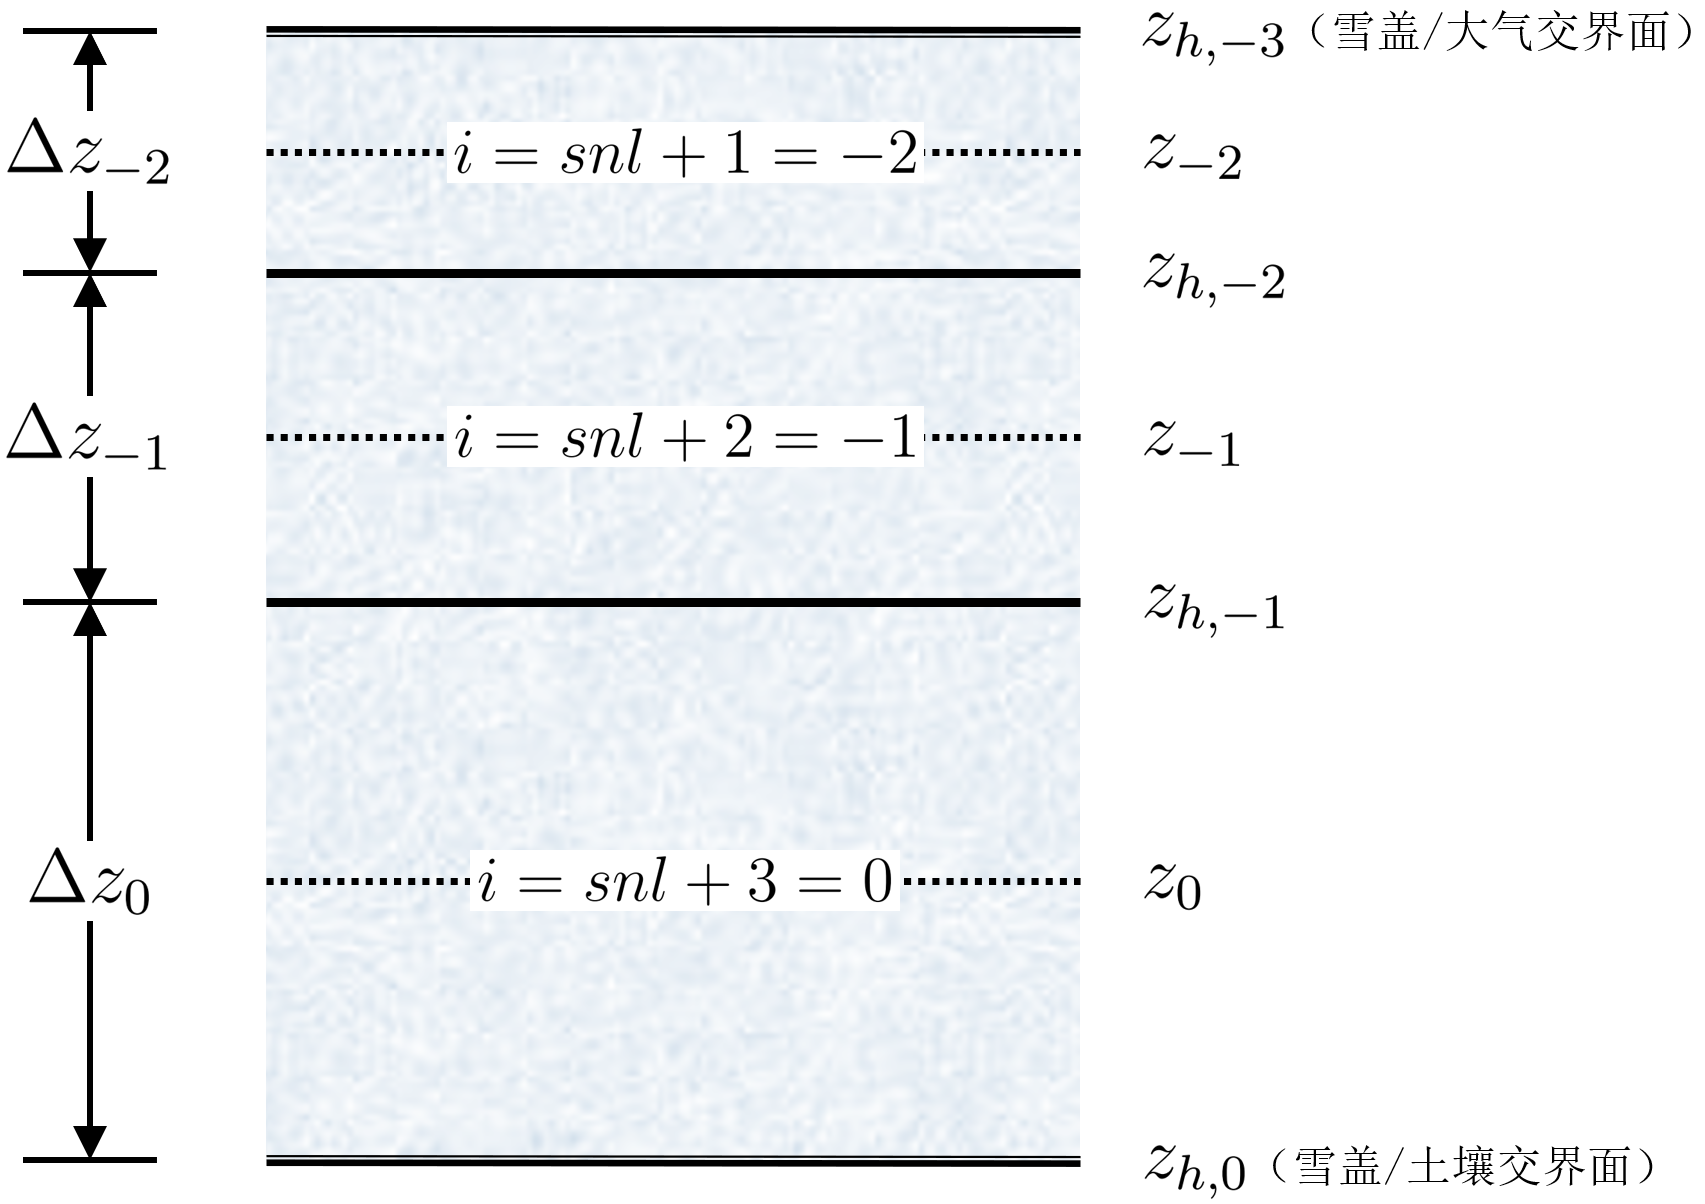
\includegraphics{Figures/雪盖土壤热力过程/模式中积雪雪层示意图.png}
\caption{模式中雪层示意图(以三层为例)}
\label{fig:模式中积雪雪层示意图}
\end{figure}
}

当固态降水$q_{sno}$的发生导致雪盖高度大于0.01 m且此时尚无雪盖分层,则将在模拟开始时创建一个新的雪层,相关物理量设置如下:
\begin{equation}
\begin{aligned}
& \Delta z_{0} &&= &{z}_{sno}& \\
& z_0 &&= &-0.5\Delta z_0& \\
& z_{h,-1} &&= &-\Delta z_0& \\
& T_0 &&= &\min \left(T_f,T_{atm}\right)& \\
& w_{ice,0} &&= &W_{sno}& \\
& w_{liq,0} &&= &0&
\end{aligned}
\end{equation}
其中$T_f$为水的冻结温度,$T_{atm}$为大气温度,$w_{ice}$和$w_{liq}$分别表示雪层中固态水的含量和液态水的含量(\unit{kg.m^{-2}})。


\subsection{雪的压实}
\begin{mymdframed}{代码}
本节对应的代码文件为\texttt{MOD\_SnowLayersCombineDivide.F90}。
\end{mymdframed}

积雪的压实主要包括以下四个过程:
\begin{enumerate}
\item 破坏变质作用(新雪的冰晶粒子在风和热力作用下树状结构的破裂),
\item 上覆积雪自重引起的压实,
\item 融化变质作用(积雪经历多次冻融循环后融雪的水出流导致雪层结构的改变),
\item 风吹雪引起的压实。
\end{enumerate}

前两个过程的处理方法分别来自 SNTHERM.99 \citep{jordan1999heat}和 SNTHERM.89 \citep{jordan1991one},融化变质的贡献取决于雪层融化过程中前后时刻固态水的变化率,风吹雪压实则考虑了下降风对雪的影响。积雪的总压实率可写为上述四个过程的和:
%
\begin{equation}
C_{R,i}=\frac{1}{\Delta {z_i}} \frac{\partial \Delta {z_i}}{\partial {t}}=C_{R1,i}+C_{R2,i}+C_{R3,i}+C_{R4,i}
\end{equation}
当雪层达到饱和
\begin{equation}
1-\left(\frac{w_{ice,i}}{ \Delta {z_i} \rho_{ice}}+\frac{w_{liq,i}}{ \Delta {z_i} \rho_{liq}}\right) \leqslant 0.001
\end{equation}
或固态水含量$w_{ice,i}\leqslant0.1$时,不再考虑雪的压实。

经过压实后雪层厚度更新为:
\begin{equation}
\Delta z_i^{n+1}=\Delta z_i^n\left(1+C_{R, i} \Delta t\right)
\end{equation}


\subsubsection{破坏变质引起的压实}
雪在到达地面后,随即快速变化。在热力作用的影响下,单个雪花原有的树状结构发生破裂,向球状结构演变。这些雪花又会和其他雪花融合生长,使雪粒之间结合得更加紧密,最终发生沉降堆积。对于密度小于 \qty{100}{kg.m^{-3}} 的新雪来说,破坏变质引起的沉降非常重要。雪粒的树状结构会使它们之间产生一种类似于“齿轮咬合”的作用,从而具有一定的强度,这种强度在破环变质的过程中会逐渐减弱。\citet{anderson1976point}对这一阶段的压实过程提出了以下经验函数:
\begin{equation}\label{eq:DestruciveCompact}
C_{R1,i}=\left[\frac{1}{\Delta {z_i}} \frac{\partial \Delta {z_i}}{\partial {t}}\right]_{\text {destructive }}=-2.777 \times 10^{-6} {c}_{3} {c}_{4} {e}^{-0.04\left(T_f-T\right)}
\end{equation}
其中
\begin{equation}
    c_3=\begin{cases}
        1 &\text{当}\ \frac{w_{ice,i}}{\Delta z_i} \leqslant 100 \;\unit{kg.m^{-3}}\text{ 时} \\
        e^{-0.046\left(\frac{w_{ice,i}}{\Delta z_i}-100\right)} &\text{当}\ \frac{w_{ice,i}}{\Delta z_i}>100 \;\unit{kg.m^{-3}}\text{ 时}
    \end{cases}
\end{equation}
\begin{equation}
    c_4=\begin{cases}
        1 &\qquad \quad \qquad \quad \;\text{当}\ \frac{w_{liq,i}}{\Delta z_i} \leqslant 0.01 \;\unit{kg.m^{-3}}\text{ 时} \\
        2 &\qquad \quad \qquad \quad \;\text{当}\ \frac{w_{liq,i}}{\Delta z_i}>0.01 \;\unit{kg.m^{-3}}\text{ 时}
    \end{cases}
\end{equation}
这两个系数表明,当雪层中固态水的体积密度超过 \qty{100}{kg.m^{-3}} 时,破环变质的速率会有所降低;当雪层中存在一定液态水时,破环变质的速率将成倍增加。

\subsubsection{雪层负重引起的压实}
随着积雪的累积,上覆积雪的自重会进一步地压实雪层。上覆雪产生的压力(负重)使雪粒粘结生长速度加快,形成更加有效的堆积形状。在经过前一过程的压实后,这一阶段的压实速率会减慢,主要和雪层的负重压力有关。在低压力范围的季节性积雪内,这一阶段的压实率是负重的线性函数\citep{anderson1976point},即
\begin{equation}\label{eq:OverburdenCompact}
C_{R2,i}=\left[\frac{1}{\Delta {z_i}} \frac{\partial \Delta {z_i}}{\partial {t}}\right]_{\text {overburden }}=-\frac{P_{s,i}}{\eta}
%=-\frac{{P}_{{s}}}{9 \times 10^{5}} {e}^{-0.08\left(T_f-{T}\right)-0.023 \rho_{{i}} \theta_{{i}}}
\end{equation}
其中$P_{s,i}$是雪层负重的质量(\unit{kg.m^{-2}}),等于其上覆雪层中固态水和液态水的质量总和加上该层自身固态水和液态水质量的一半,即
\begin{equation}
P_{s,i}=\frac{w_{ice,i}+w_{liq,i}}{2}+\sum_{{j}={snl}+1}^{{j}={i}-1}\left({w}_{ice,j}+{w}_{liq,j}\right)
\end{equation}
~\eqref{eq:OverburdenCompact} 式中变量$\eta$为粘滞系数(\unit{kg.s.m^{-2}}),与雪层的密度和温度有关:
\begin{equation}
    \eta=f_1 f_2 \eta_0 \frac{\rho_i}{c_\eta} e^{a_\eta \left(T_f-T_i\right)+b_\eta \rho_i}
\end{equation}
其中$\rho_i=\frac{w_{ice,i}}{\Delta z_i}$为雪层中固态水的体积密度,常系数$\eta_0=7.62237 \times 10^6$ \unit{kg.s^{-1}.m^{-2}},$a_\eta=0.1$ \unit{K^{-1}},$b_\eta=0.023$ \unit{m^{-3}.kg^{-1}},$c_\eta=450$ \unit{kg.m^{-3}} \citep{Kampenhout2017}。系数$f_1$和雪层中液态水的含量有关~\citep{Vionnet2012}:
\begin{equation}
    f_1=\frac{1}{1+60\frac{w_{liq,i}}{\rho_{liq}\Delta z_i}}
\end{equation}
系数$f_2$则与雪层中棱状雪粒(angular grains)的含量有关,目前的计算中固定$f_2=4$。

\subsubsection{雪层融化引起的压实}
在融雪过程的后期(积雪经过多次冻融循环后),融雪水的出流导致雪堆更加致密,雪层产生压实。这一阶段的压实率取决于雪层融化过程中前后两个时间步数固态水的变化率
\begin{equation}
C_{R3,i}=\left[\frac{1}{\Delta {z_i}} \frac{\partial \Delta {z_i}}{\partial {t}}\right]_{melt}=-\frac{1}{\Delta {t}}\max\left(0,\frac{{f}_{{ice,i}}^{n}-{f}_{{ice,i}}^{n+1}}{{f}_{ice,i}^{n}}\right)
\end{equation}
其中$f_{ice,i}=w_{ice,i}/\left({w_{ice,i}+w_{liq,i}}\right)$为雪层中固态水占全部水含量的比例。

\subsubsection{风吹雪引起的压实}
在高纬的冰原地区,低温使破坏变质的过程发生缓慢,此时高速的下降风将占据主导,气流使雪粒的树状结构破碎,引发雪粒堆积,产生压实。在这种情况下,引入风吹雪压实的参数化方案~\citep{Vionnet2012}:
\begin{equation}
    C_{R4,i}=\left[\frac{1}{\Delta z_i}\frac{\partial \Delta z_i}{\partial t}\right]_{drift}=-\frac{\max \left(0,\rho_{\text{max}}-\rho_i\right)}{\tau_i}
\end{equation}
其中,$\rho_{\text{max}}=350$ \unit{kg.m^{-3}}是这一过程的有效密度上限,$\tau_i$是一个与雪层深度有关的时间尺度变量:
\begin{equation}
    \tau_i=\frac{\tau}{\Gamma_{\text{drift}}^i}, \quad \Gamma_{\text{drift}}^i=\max \left(0,S_I^i e^{-z_i/0.1}\right)
\end{equation}
常数$\tau$是风吹雪压实过程的一个特征时间尺度,根据经验被设置为48 \unit{h},$z_i=\sum_j \Delta z_j \cdot \left(3.25-S_I^j\right)$称为伪深度,与当前雪层$i$上方的$j$个雪层的硬化程度有关。$S_I$称为吹雪飘移指数(driftability index):
\begin{equation}
    S_I=-2.868 e^{-0.085 U} + 1 + M_O
\end{equation}
其由10 \unit{m}风速$U$和雪的流动指数(mobility index)$M_O$共同作用,反映了雪粒在风的作用下受到的飘移影响。雪的流动指数
\begin{equation}
    M_O=0.34\left(-0.583g_s-0.833s+0.833\right)+0.66F\left(\rho\right)
\end{equation}
与雪的微观结构有关,描述了雪层受侵蚀的可能性,其中
$$F\left(\rho\right)=1.25-0.0042 \cdot \\\left[\max \left(\rho_{min},\rho\right)-\rho_{min}\right],$$$\rho_{min}=50$ \unit{kg.m^{-3}}。$g_s$和$s$是两个和雪粒形态有关的变量,$s$称为雪粒的球度(sphericity),从0 -- 1不等,$g_s$为雪粒大小,一般为0.3至0.4 \unit{mm}。


\subsection{雪层的合并}
\begin{mymdframed}{代码}
本节对应的代码文件为\texttt{MOD\_SnowLayersCombineDivide.F90}。
\end{mymdframed}

在进行雪层的合并前,先自上而下遍历所有雪层,当任何一层几近融化(即$w_{ice,i} \leqslant 0.1$ \unit{kg.m^{-2}})时,移除该雪层,且将其液态水和固态水含量分配到与之相邻的下层中:
\begin{equation}
    w_{liq,i+1} = w_{liq,i+1} + w_{liq,i}
\end{equation}
\begin{equation}
    w_{ice,i+1} = w_{ice,i+1} + w_{ice,i}
\end{equation}
这也包括了与土壤相邻的底层雪层,该层的液态水和固态水含量将直接被分配到土壤层顶层中。每移除一层雪层,该层以上的雪层编号将增加1,该层以下的雪层编号保持不变,以对应新的雪盖分层。

如果已无雪层存在($snl=0$),雪水当量$W_{sno}$和雪盖高度$z_{sno}$将被设为0。如果仍有雪层存在,则$W_{sno}$和$z_{sno}$根据下式更新为
\begin{equation}
    W_{sno} = \sum_{i=snl+1}^{i=0}\left(w_{ice,i}+w_{liq,i}\right)
\end{equation}
\begin{equation}
    z_{sno} = \sum_{i=snl+1}^{i=0} \Delta z_i
\end{equation}
若雪盖高度$z_{sno} < 0.01$ \unit{m},则雪盖层数$snl$仍被设为0,此时雪水当量
$$W_{sno}=\sum_{i=snl+1}^{i=0} w_{ice,i}$$
将仅计算雪盖固态水含量,雪盖液态水含量$\sum_{i=snl+1}^{i=0} w_{liq,i}$将分配给土壤层顶层。

当某一雪层的厚度$\Delta z_i$小于规定的最小值$\Delta z_{min}$时,则将该雪层与相邻雪层合并。如果该雪层:
\begin{enumerate}
\item 为顶层,则与相邻的下层雪层合并;
\item 为底层(与土壤相邻),则与相邻的上层雪层合并;
\item 不为上述雪层,则与厚度较薄的相邻雪层合并。
\end{enumerate}

五个雪层(从顶层到底层)规定的厚度最小值$\Delta z_{min}$分别为 0.010、0.015、0.025、0.055 和 0.115(\unit{m})。

当两个雪层(这里用编号1和2表示)合并时,合并层的厚度为
\begin{equation}\label{eq:SnowCombThick}
\Delta {z}_c=\Delta {z}_{1}+\Delta {z}_{2}
\end{equation}
根据质量守恒,合并层的质量计算为
\begin{equation}
w_{liq,c}=w_{liq,1}+w_{liq,2}
\end{equation}
\begin{equation}
w_{ice,c}=w_{ice,1}+w_{ice,2}
\end{equation}
根据焓变守恒,合并层的温度计算为
\begin{equation}\label{eq:SnowCombTemp}
T_c=\begin{cases}
    T_f+{h_c}/\left(C_{ice}w_{ice,c}+C_{liq}w_{liq,c}\right) &\text{当}\ h_c<0 \text{ 时} \\
    T_f &\text{当}\ 0 \leqslant h_c \leqslant L_f w_{liq,c} \text{ 时}\\
    T_f+\left(h_c-L_f w_{liq,c}\right)/\left(C_{ice} w_{ice,c}+C_{liq} w_{liq,c}\right) &\text{当}\ h_c > L_f w_{liq,c} \text{ 时}
\end{cases}
\end{equation}
其中$h_c=h_1+h_2$为两个雪层合并后的焓,雪层$i$的焓$h_i$可通过以下公式得出
\begin{equation}
    h_i=\left(C_{ice}w_{ice,c}+C_{liq}w_{liq,c}\right)\left(T_i-T_f\right)+L_fw_{liq,i}
\end{equation}
$L_f$为融化潜热(\unit{J.kg^{-1}}),$C_{liq}$和$C_{ice}$分别为液态水和固态水的比热容(\unit{J.kg^{-1}.K^{-1}})。

计算完雪层的合并后,根据下式更新雪层深度和雪层交界面深度
\begin{equation}
    z_i=z_{h,i}-0.5\Delta z_i \;\;\;\;\;i=0,\;...,\;snl+1
\end{equation}
\begin{equation}
    z_{h,i-1}=z_{h,i}-\Delta z_i \;\;\;\;\;i=0,\;...,\;snl+1
\end{equation}
其中$\Delta z_i$为雪层厚度。



\subsection{雪层的细分}
当某一雪层的厚度$\Delta z_i$大于规定的最大值$\Delta z_{max}$时,雪层将被细分。最大厚度$\Delta z_{max}$和雪盖的层数有关。例如,如果雪盖只被分为一层,那么顶层(可以这么称)的最大厚度将为0.03 \unit{m};如果雪盖被分为多层,那么顶层的最大厚度则为0.02 \unit{m}。

如果被细分的雪层为底层,则将该雪层等分为厚度相等的两层,并均分液态水含量和固态水含量,温度和原雪层保持一致,此时雪盖层数$snl$将增加1。如果被细分的雪层不为底层,先将该层细分为上下两层,其中上层雪层的厚度限为该层的规定最大厚度$\Delta z_{max}$,下层雪层的厚度则为$\Delta z_i - \Delta z_{max}$,原雪层的液态水含量和固态水含量按厚度比例分配给上下两个雪层,温度在细分前后保持不变,再将下层雪层作为多余部分根据式~\eqref{eq:SnowCombThick} -~\eqref{eq:SnowCombTemp}和原雪层的相邻下层雪层合并,从而保证雪盖层数$snl$不变。不同情况雪层的最大厚度如表~\ref{lab:雪层最大厚度} 所示。

\begin{table}[!ht]
    \centering
    \caption{不同雪盖层数下每层雪层的最大厚度}
    \label{lab:雪层最大厚度}
    \begin{tabular}{c|c|c|c|c}
    \toprule
        雪盖层数 & $N_{l}$ & $N_{u}$ & $(\Delta z_{max})_{l}$ & $(\Delta z_{max})_{u}$ \\ \midrule
        1 & 1 & >1 & 0.03 & 0.02 \\
        2 & 2 & >2 & 0.07 & 0.05 \\
        3 & 3 & >3 & 0.18 & 0.11 \\
        4 & 4 & >4 & 0.41 & 0.23 \\
        5 & 5 & 5 & 无限制 & 无限制 \\ \bottomrule
    \end{tabular}
\end{table}


\subsection{雪盖的水量平衡}
\begin{mymdframed}{代码}
本节对应的代码文件为\texttt{MOD\_SoilSnowHydrology.F90}。
\end{mymdframed}

雪盖的液态水质量守恒方程为
\begin{equation}
    \frac{\partial w_{liq,i}}{\partial t}=\left(q_{liq,i-1}-q_{liq,i}\right)+\frac{{\left(\Delta w_{liq,i}\right)}_p}{\Delta t}
\end{equation}
其中$q_{liq,i-1}$表示第$i-1$层流入至第$i$层的液态水,$q_{liq,i}$表示第$i$层流出至第$i+1$层的液态水,${{\left(\Delta w_{liq,i}\right)}_p}/{\Delta t}$表示由于相态变化导致的水量改变率(见章节\textcolor{red}{??})。对于雪盖顶层,需先考虑固态水的变化导致的液态水改变。由于升华和凝华作用,雪盖顶层固态水的变化为
\begin{equation}
    w_{ice,snl+1}^{n+1}=w_{ice,snl+1}^n+\left(q_{frost}-q_{subl}\right)\Delta t
\end{equation}
其中$q_{subl}$和$q_{frost}$分别表示水的升华和凝华速率(\unit{kg.m^{-2}.s^{-1}}或 \unit{mm.H_2O.s^{-1}})。如果$w_{ice,snl+1}^{n+1}<0$,将固态水含量重置为0,并从液态水中减去固态水增加到0所需的水含量。雪盖顶层的$q_{liq,i-1}$则由以下公式计算
\begin{equation}
    q_{liq,i-1}=q_{grnd,liq}+\left(q_{sdew}-q_{seva}\right)
\end{equation}
其中$q_{grnd,liq}$为到达雪盖的液态降水速率,$q_{seva}$和$q_{sdew}$分别表示水的蒸发和凝结速率。基于此,顶层液态水含量更新为
\begin{equation}w_{liq,snl+1}^{n+1}=w_{liq,snl+1}^n+\left(q_{grnd,liq}+q_{sdew}-q_{seva}\right)\Delta t
\end{equation}

当液态水含量超过了雪层的最大持水量时,多余的液态水将下渗到相邻雪层,渗透能力取决于雪层的有效孔隙度($1-\theta_{ice}$)。如果两层中任一层有效孔隙度($1-\theta_{ice,i}$和$1-\theta_{ice,i+1}$)小于不透水体积含水量$\theta_{imp}=0.05$,则假定两层间液态水流量为0。所以,对于雪层$i=snl+1,\ ...,\ 0$,液态水流量$q_{liq,i}$被计算为
\begin{equation}
    q_{liq,i}=\frac{\rho_{liq}\left[\theta_{liq,i}-S_r\left(1-\theta_{ice,i}\right)\right]\Delta z_i}{\Delta t}\geqslant 0
\end{equation}
其中固态水和液态水的体积含水量分别为
\begin{align}
    \theta_{ice,i}&=\frac{w_{ice,i}}{\Delta z_i \rho_{ice}} \leqslant 1 \\
    \theta_{liq,i}&=\frac{w_{liq,i}}{\Delta z_i \rho_{ice}} \leqslant 1-\theta_{ice,i}
\end{align}
$S_r=0.033$称为束缚水饱和度(由于毛细管的滞留作用,渗透结束后雪层仍会保留一定含量的液态水)。$q_{liq,i}$同时也受到相邻下层最大持水量的限制,除非其相邻下层为土壤层,即
\begin{equation}
    q_{liq,i} \leqslant \frac{\rho_{liq}\left(1-\theta_{ice,i+1}-\theta_{liq,i+1}\right)\Delta z_{i+1}}{\Delta t} \qquad i=snl+1,\ ...,\ -1
\end{equation}
最后,液态水含量更新为
\begin{equation}\label{eq:SnowWater}
    w_{liq,i}^{n+1}=w_{liq,i}^n+\left(q_{i-1}-q_i\right)\Delta t
\end{equation}
对于每个时间步长,依次从雪盖顶层到底层计算式~\eqref{eq:SnowWater}。到达土壤层的液态水即为$q_{liq,0}$,被用于地表径流和下渗的计算当中。

\subsection{雪盖的黑碳、有机碳和矿物粉尘}
由于大气的气溶胶沉降,积雪中会存在一定的颗粒物,影响雪盖的辐射传输。雪中颗粒物含量仅以质量守恒作为简单约束,这部分的计算均被定义在SNICAR模型中。对于每个雪层,该模型包括了以下八种颗粒物的含量,亲水性黑碳、疏水性黑碳、亲水性有机碳、疏水性有机碳和四种矿物粉尘(颗粒半径分别为0.1-1.0,1.0-2.5,2.5-5.0,5.0-10.0 \unit{\mu m})。每种颗粒物都具有不同的光学属性和融水清除率。

黑碳和有机碳的沉降率被分为以下四类
\begin{align}
    D_{bc,hphob}&=D_{bc,dryphob} \\
    D_{oc,hphil}&=D_{oc,dryhphil}+D_{oc,wethphil} \\
    D_{bc,hphil}&=D_{bc,dryhphil}+D_{bc,wethphil} \\
    D_{oc,hphob}&=D_{oc,dryphob}
\end{align}

假定沉降的颗粒物立即在表面雪层中均匀混合,并在计算雪层层间液态水通量之后添加,以使沉降后的一些气溶胶颗粒位于顶层,并且在进行反照率相关的计算之前不会被冲走。对于每个时间步长,在进行雪层间液态水流动以及雪层的合并和细分计算中,都将根据质量守恒更新每层颗粒物含量。每种颗粒物种的质量变化$\Delta m_{sp,i}$为
\begin{equation}
    \Delta m_{sp,i}=\left[k_{sp}\left(q_{liq,i-1} c_{sp,i-1}-q_{liq,i} c_i\right)+D_{sp}\right] \Delta t
\end{equation}
其中$k_{sp}$表示每种颗粒物的融水清除率,具体参见表~\ref{lab:融水清除率}。$c_{sp,i-1}$和$c_{sp,i}$分别表示$i-1$层和$i$层的颗粒物质量混合比(\unit{kg.kg^{-1}}),$D_{sp}$表示大气气溶胶沉降率(仅在$snl+1$层考虑)。颗粒物质量混合比为
\begin{equation}
    c_{i}=\frac{m_{sp,i}}{w_{liq,i}+w_{ice,i}}
\end{equation}

$k_{sp}$的具体值根据~\citet{Conway2012}等人的实验得出。雪盖底层被融水带走的颗粒物被认为从雪盖中永久消失,模式中不再考虑。

\begin{table}[!ht]
    \centering
    \caption{雪盖中不同颗粒物的融水清除率}
    \begin{tabular}{l|c}
    \toprule
        颗粒种类 & $k_{sp}$ \\ \midrule
        亲水性黑碳 & 0.20 \\
        疏水性黑碳 & 0.03 \\
        亲水性有机碳 & 0.20 \\
        疏水性有机碳 & 0.03 \\
        1类矿物粉尘(0.1-1.0 \unit{\mu m}) & 0.02 \\
        2类矿物粉尘(1.0-2.5 \unit{\mu m}) & 0.02 \\
        3类矿物粉尘(2.5-5.0 \unit{\mu m}) & 0.01 \\
        4类矿物粉尘(5.0-10.0 \unit{\mu m}) & 0.01 \\ \bottomrule
    \end{tabular}
    \label{lab:融水清除率}
\end{table}

